\title{Hash}

\frame{\maketitle}

\begin{frame}{Acesso direto}


\tikzset{>=latex,every node/.style={font=\footnotesize}}

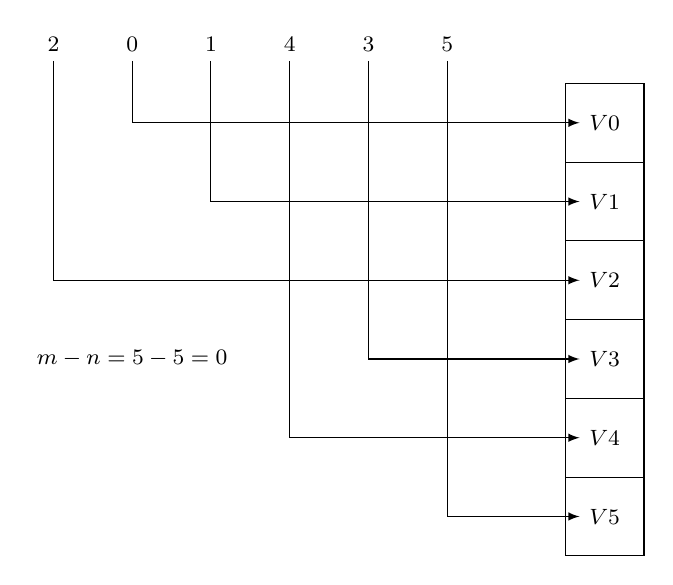
\begin{tikzpicture}
    \foreach \x/\k in {0/2,1/0,2/1,3/4,4/3,5/5}{
    	     \node (key\k) at (\x,0) {$\k$};
       	     \node (vec\x) at (7,-1-\x) {$V\x$};
	     \draw (7,-1-\x) +(-.5,-.5) rectangle ++(.5,.5);
    }
    
    \foreach \i in {0,1,2,3,4,5}{
    	     \path[->,draw] (key\i)-- +(0,-1-\i) -- (vec\i.west);
    }
    
    \node at (1,-4) {$m-n=5-5=0$};
\end{tikzpicture}

\end{frame}

\begin{frame}{Acesso direto}

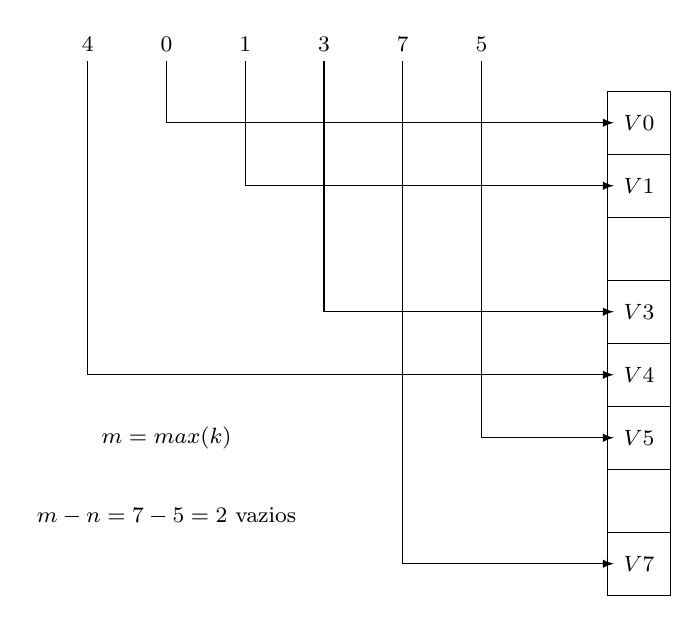
\begin{tikzpicture}
    \foreach \x/\k in {0/4,1/0,2/1,3/3,4/7,5/5}{
    	     \node (key\k) at (\x,0) {$\k$};
    }
    \foreach \x/\v in {0/V0,1/V1,2/,3/V3,4/V4,5/V5,6/,7/V7}{
       	     \node (vec\x) at (7,-1-\x*.8) {$\v$};
	     \draw (7,-1-\x*.8) +(-.4,-.4) rectangle ++(.4,.4);
    }
    \foreach \i in {0,1,3,4,5,7}{
    	     \path[->,draw] (key\i)-- +(0,-1-\i*.8) -- (vec\i.west);
    }
    \node (max) at (1,-5) {$m=max(k)$};
    \node [below of=max] {$m-n=7-5=2$ vazios};
\end{tikzpicture}

\end{frame}

\begin{frame}{Hash}

\noindent $m-n$ deve ser pequeno para evitar grande número de compartimentos
 vazios, ou seja, desperdício de memória.\bigskip

\noindent Caso limite: $m=999.999$, $n=0$\bigskip\pause

\noindent \alert{Solução}: Mapear a chave $k$ em um intervalo $0\leq k\leq m-1$
através de uma função de espalhamento ({\it hash}) \alert{$h(k)$}.\bigskip\pause

\noindent \alert{$h(k)$}: índice de $k$, se o compartimento $h(k)$ não estiver ocupado,
preencher com o valor associado à chave $k$.

\end{frame}

\begin{frame}{Hash}

\noindent Porém, $h(k)$ não garante injetividade.\bigskip

\begin{center}
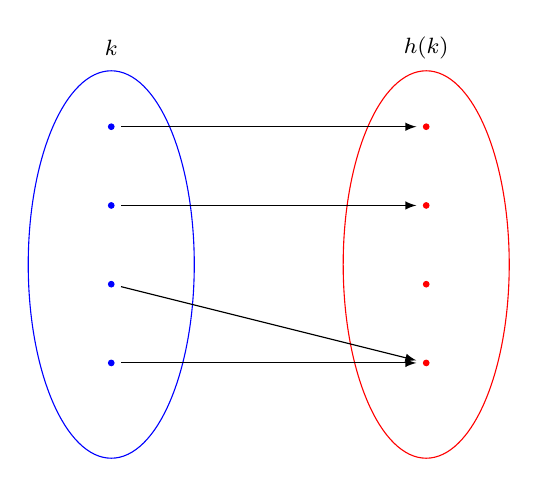
\begin{tikzpicture}

    \foreach \i in {0,1,2,3}{
    	     \draw<1>[blue,fill] (0,-\i) circle (1pt);
	     \node<1> (x\i) at (0,-\i) {};
    }
    \draw<1>[blue] (0,-1.75) ellipse (30pt and 70pt);

    \foreach \i in {0,1,2,3}{
    	     \draw<1>[red,fill] (4,-\i) circle (1pt);
     	     \node<1> (y\i) at (4,-\i) {};
    }
    \draw<1>[red] (4,-1.75) ellipse (30pt and 70pt);

    \foreach \x/\y in {0/0,1/1,2/3,3/3}{
    	     \draw<1>[->] (x\x) -> (y\y);
    }
    \node<1> at (0,1) {$k$};
    \node<1> at (4,1) {$h(k)$};
\end{tikzpicture}

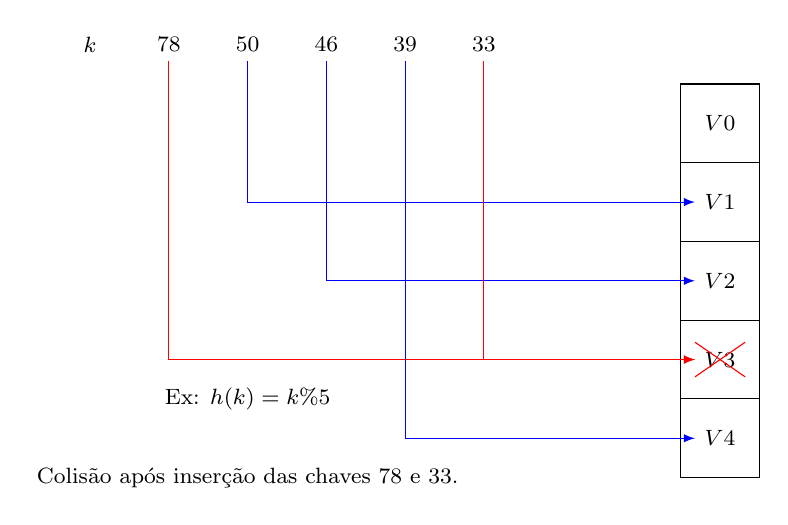
\begin{tikzpicture}
    \foreach \x/\k in {0/78,1/50,2/46,3/39,4/33}{
    	     \node<2-> (key\x) at (\x,0) {$\k$};
       	     \node<2-> (vec\x) at (7,-1-\x) {$V\x$};
	     \draw<2-> (7,-1-\x) +(-.5,-.5) rectangle ++(.5,.5);
    }
    
    \foreach \ki/\vi/\color in {0/3/red,1/1/blue,2/2/blue,3/4/blue,4/3/red}{
    	     \path<2->[->,draw=\color] (key\ki)-- +(0,-1-\vi) -- (vec\vi.west);
    }

    \node<2-> at (-1,0) {$k$};

    \draw<2->[red] (vec3.north east) -- (vec3.south west);
    \draw<2->[red] (vec3.north west) -- (vec3.south east);
    
    \node<2-> (h) at (1,-4.5) {Ex: $h(k)=k \% 5$};

    \node<3> [below of=h] {Colisão após inserção das chaves $78$ e $33$.};
\end{tikzpicture}
\end{center}

\end{frame}


\begin{frame}{Funções de hash}

Propriedades desejáveis:

\begin{itemize}
\item Produzir um número baixo de colisões;
\item Ser facilmente computável;
\item Ser uniforme.
\end{itemize}

\end{frame}

\begin{frame}{Funções de hash}

Normalmente é utilizada a função \alert{módulo resto} ($mod$).

\[ h(k) = k mod\ M, \qquad 0\leq h(k)<M\]

\pause

\noindent Escolha de $M$:

- $M$ deve ser ímpar;
- $M$ seja \alert{primo}, para evitar colisões devido à divisibilidade dos
múltiplos de $M$.

\end{frame}

\def\NULL#1{
  \node[on chain,draw,inner sep=6pt] (N#1)[right of=#1]{};
  \draw (N#1.north east) -- (N#1.south west);
  \draw (N#1.north west) -- (N#1.south east);
  \draw[*->] let \p1 = (#1.two), \p2 = (#1.center) in (\x1,\y2) -- (N#1);
}

\def\EMPTYKEY#1{
  \node[on chain,draw,inner sep=6pt] (E#1)[right of=#1]{};
  \draw (E#1.north east) -- (E#1.south west);
  \draw (E#1.north west) -- (E#1.south east);
  \draw[*->] (#1) -- (E#1);
}


\begin{frame}{Resolução de colisões: encadeamento (chaining)}

\begin{tikzpicture}[list/.style={rectangle split, rectangle split parts=2,
    draw, rectangle split horizontal}, >=stealth, start chain]

   \foreach \i in {0,1,2,3,4,5,6}{
    	     \node at (-1,-\i) {$\i$};
	     \draw (0,-\i) +(-.5,-.5) rectangle ++(.5,.5);
	     \node (K\i) at (0,-\i) {};
  }


  \node[list,on chain] (A) [right of=K0,xshift=1cm]{``CPF''};
  \node[list,on chain] (B) [right of=K2]{``assim``};
  \node[list,on chain] (C) [right of=B]{``missa''};
  \node[list,on chain] (D) [right of=K5]{``de''};
  \node[list,on chain] (E) [right of=K6]{``que''};

  \draw[*->] (K0) -- (A);
  \NULL{A}

  \EMPTYKEY{K1}
  
  \draw[*->] (K2) -- (B);
  \draw[*->] let \p1 = (B.two), \p2 = (B.center) in (\x1,\y2) -- (C);
  \NULL{C}

  \EMPTYKEY{K3}
  \EMPTYKEY{K4}
  
  \draw[*->] (K5) -- (D);
  \NULL{D}

  \draw[*->] (K6) -- (E);
   \NULL{E}

   \node<2->[] (D) [right of=K3,xshift=6cm] {taxa de ocupação: $d= {N\over M} = {4\over 7}=0,57=57\%$};
   \node<3> (alpha) [below of=D]{fator de carga: $\alpha={NN\over M}={5\over 7}=0,714=71,4\%$}; 

\end{tikzpicture}

\end{frame}


\begin{frame}{Fluxograma}

\begin{tikzpicture}[every node;/.style={font=\scriptsize}]
\tikzstyle{process} = [rectangle, minimum width=1.5cm, minimum height=.7cm, text width=1.5cm,
		    text centered, draw=black, fill=orange!30]
\tikzstyle{decision} = [diamond, minimum width=3cm, minimum height=.7cm, text centered, draw=black, fill=green!30]
\tikzstyle{arrow} = [thick,->,>=latex]

\node[process] (H1) {H1. Hash};
\node[process] (H2) [below of=H1,yshift=-1cm]{H2. Está na lista?};
\node[decision] (H3) [below of=H2,yshift=-1.5cm]{H3. Compara};
\node[process] (H4) [right of=H3,xshift=2cm]{H4. Avance para o próximo};
\node[process] (H5) [right of=H4,xshift=2cm]{H5. Ache nó vazio};
\node[process] (H6) [right of=H5,xshift=2cm]{H6. Insere nova chave};
\node (S) [below of=H3,yshift=-1.5cm]{Sucesso};

\draw[arrow] (H1) -- (H2);
\draw[arrow] (H2) -- node[right] {sim}  (H3);
\draw[arrow] (H3) -- (H4);
\draw[arrow] (H3) -- node[right] {\tt k=key[i]} (S);
\draw[arrow] (H4) -- (H5);
\draw[arrow] (H5) -- (H6);
\draw[arrow] (H2) node[anchor=south west] [xshift=1cm]{não} -- +(9,0) -- (H6);

\end{tikzpicture}

\end{frame}

\begin{frame}[fragile]{Implementação}

\noindent {\color{blue} Estrutura de dados:}\bigskip

\begin{lstlisting}
struct lista {
        int chave;
        struct lista *prox; /* ponteiro para proximo elemento */
};
#define M 769 /* numero primo */
struct hash_table {
        struct lista *tabela[M]; /* elementos da tabela */
        int n; /* nos ocupados */
        int nn; /* numero de nos na tabela */
};
\end{lstlisting}

\end{frame}


\begin{frame}[fragile]{Implementação}


\noindent {\color{blue}Principais operações:}\bigskip

\begin{lstlisting}
struct hash_table *criar(); /* cria uma tabela de espalhamento */
void inserir(struct hash_table *tab, int chave);
int buscar(struct hash_table *tab, int chave);
void reciclar(struct hash_table **tab); /* libera memoria utilizada pela tabela */
\end{lstlisting}

\end{frame}

